\subsection{超大数据集中的数据挖掘——流形学习}
\begin{frame}{范例:超大数据集中的数据挖掘——流形学习\footnote{Barter Edmund and Gross Thilo 2019 Manifold cities: social variables of urban areas in the UK, Proc. R. Soc. A. 4752018061520180615 http://doi.org/10.1098/rspa.2018.0615}}

\begin{itemize}
    \item 从认知、规划等角度来讲,城市空间都不是一个典型的欧氏空间:同样的欧氏距离下,穿不穿越河流、人流密集还是稀疏,都会产生不同的时间消耗和其他感知差异。这个事实说明城市空间的刻画是复杂的,全局的空间度量很难刻画城市空间的本质。为了更好的描述城市空间,我们需要更复杂的城市认知框架。数学上基于局部距离定义的\textit{流形}提供了一个可能的方案。
    \pause
    \vspace{1cm}
    \item 问题:给定一个大型普查数据集,如英国普查数据集总共调查181,408个Output areas (OAs)的1450个特征。将所有的人口普查单元上的1450个特征作为行向量,所有的普查单元作为列向量,构成一个矩阵$A$。如何找到由同一个因素塑造空间模式?
\end{itemize}
\end{frame}

\begin{frame}{范例:超大数据集中的数据挖掘——流形学习}

    \begin{itemize}
        \item \textbf{找到普查规律的主要贡献变量}。
    \end{itemize}
    
    \vspace{0.5cm}
    \begin{enumerate}
    \item 将矩阵$A$进行列标准化;
    \item 将$A$的每一行作为一个向量,求矩阵两两行之间的欧氏距离,作为区域之间邻接矩阵的边权重;
    \item 以一个阈值$p$, 将权重过低的边去掉,得到截断Laplace矩阵$L$;
    \item 对矩阵$L$求特征值和特征向量,并以最小的正特征向量作为每个人口普查单元的权重,得到扩散映射的结果。
\end{enumerate}

\vspace{0.5cm}
该方法找到了最小的两个特征值对应的特征向量指示的部分英国城市最重要的贡献指标:大学生和教员的密度,以及保障性住房的空间分布。
\end{frame}

\begin{frame}{范例:超大数据集中的数据挖掘——流形学习}
    \begin{figure}
        \centering
        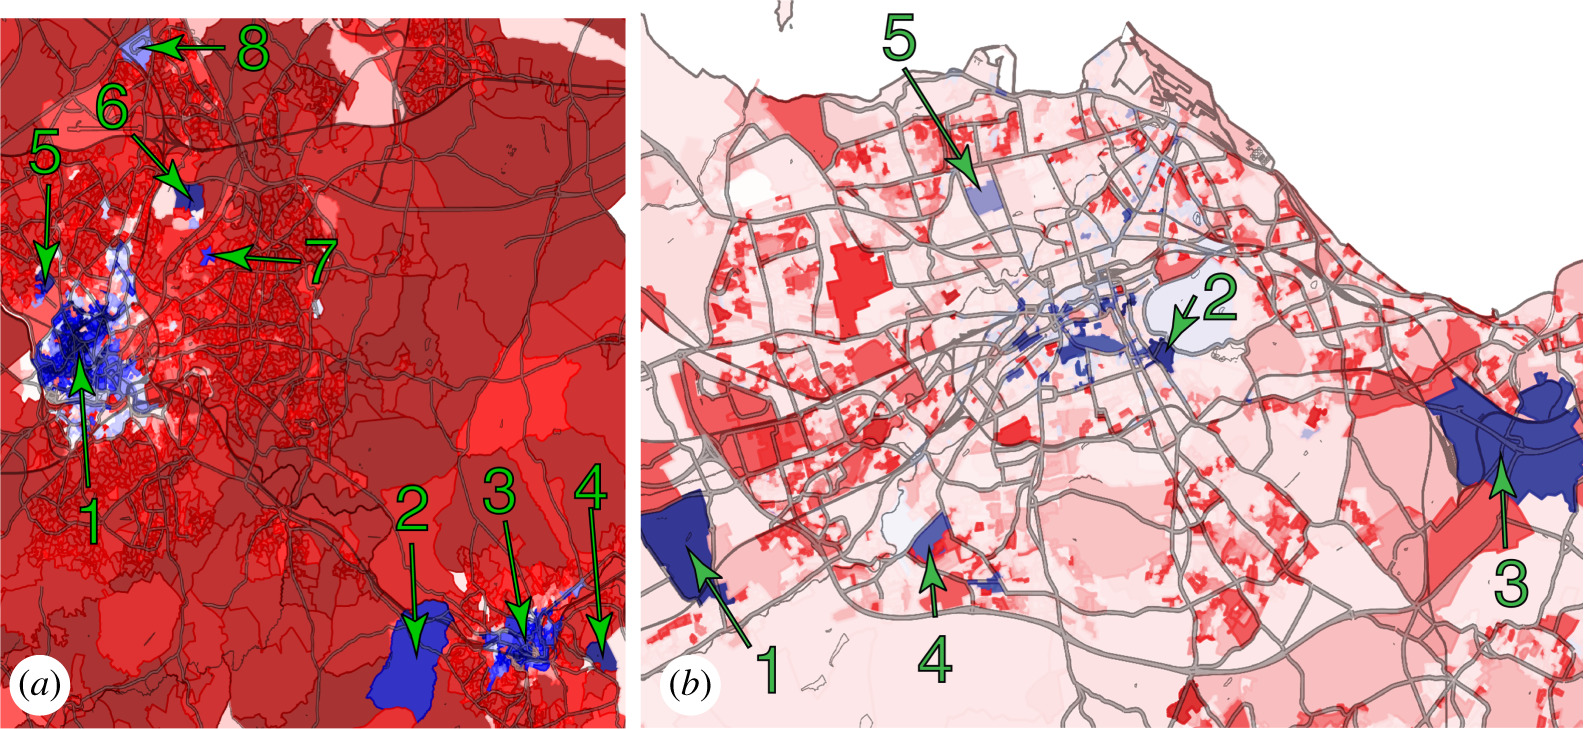
\includegraphics[width = 0.65\linewidth]{PKU_Slide/chaps/rspa20180615f02.jpg}
        \caption{Diffusion eigenvectors locate the student population in Bristol and Edinburgh. (a) The smallest positive eigenvector of the diffusion map is plotted on a map of Bristol using a colour scale from red (most negative entries) via white to blue (most positive entries). High values of the eigenvector occur in areas with a dense student population including University of Bristol and Bristol city centre (Barter Edmund and Gross Thilo 2019 Manifold cities: social variables of urban areas in the UK, Proc. R. Soc. A.)}
        % \label{fig:my_label}
    \end{figure}
\end{frame}

\begin{frame}{范例:超大数据集中的数据挖掘——流形学习}
    \begin{figure}
        \centering
        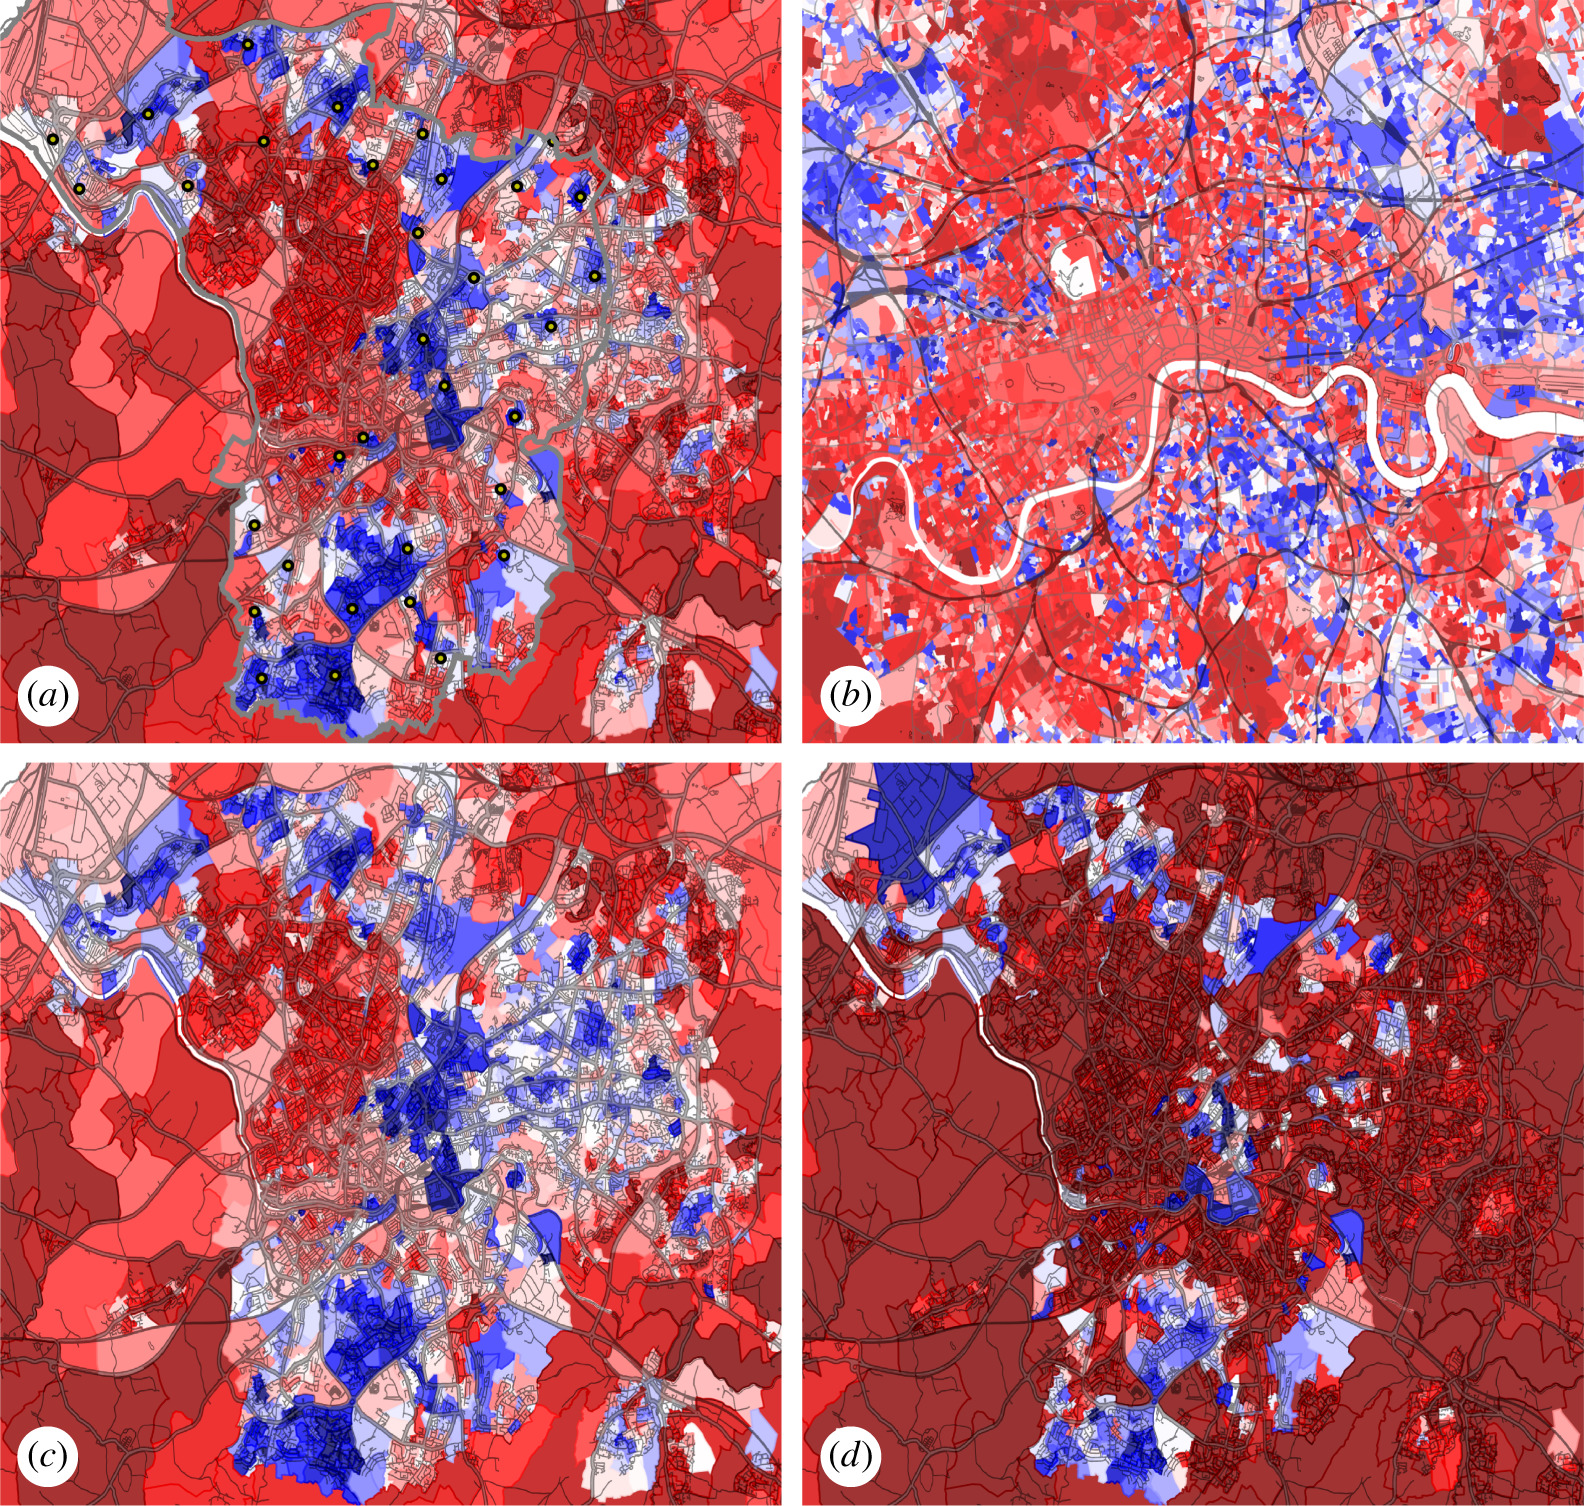
\includegraphics[width = 0.35\linewidth]{PKU_Slide/chaps/rspa20180615f03.jpg}
        \caption{The second diffusion eigenvector is an indicator of poverty. (a) Colour-coding the second smallest positive diffusion eigenvector in Bristol highlights areas (blue) that coincide locations of social housing estates (yellow dots). Dots are based on a report that covered only the Bristol unitary authority area (grey border), hence social housing estates in the rightmost part of the map are picked up by the eigenvector but not marked with a dot.  (Barter Edmund and Gross Thilo 2019 Manifold cities: social variables of urban areas in the UK, Proc. R. Soc. A.)}
        % \label{fig:my_label}
    \end{figure}
\end{frame}

\begin{frame}{方法概括:扩散映射}
\begin{itemize}
    \item Coifman R R, Lafon S, Lee A B, et al. Geometric diffusions as a tool for harmonic analysis and structure definition of data: Diffusion maps[J]. Proceedings of the national academy of sciences, 2005, 102(21): 7426-7431.
    \item Coifman R R, Lafon S. Diffusion maps[J]. Applied and computational harmonic analysis, 2006, 21(1): 5-30.
    \item Moon K R, van Dijk D, Wang Z, et al. Visualizing structure and transitions in high-dimensional biological data[J]. Nature biotechnology, 2019, 37(12): 1482-1492.
\end{itemize}
\end{frame}

\subsection{PHATE}
\begin{frame}{PHATE}
    \begin{figure}
        \centering
        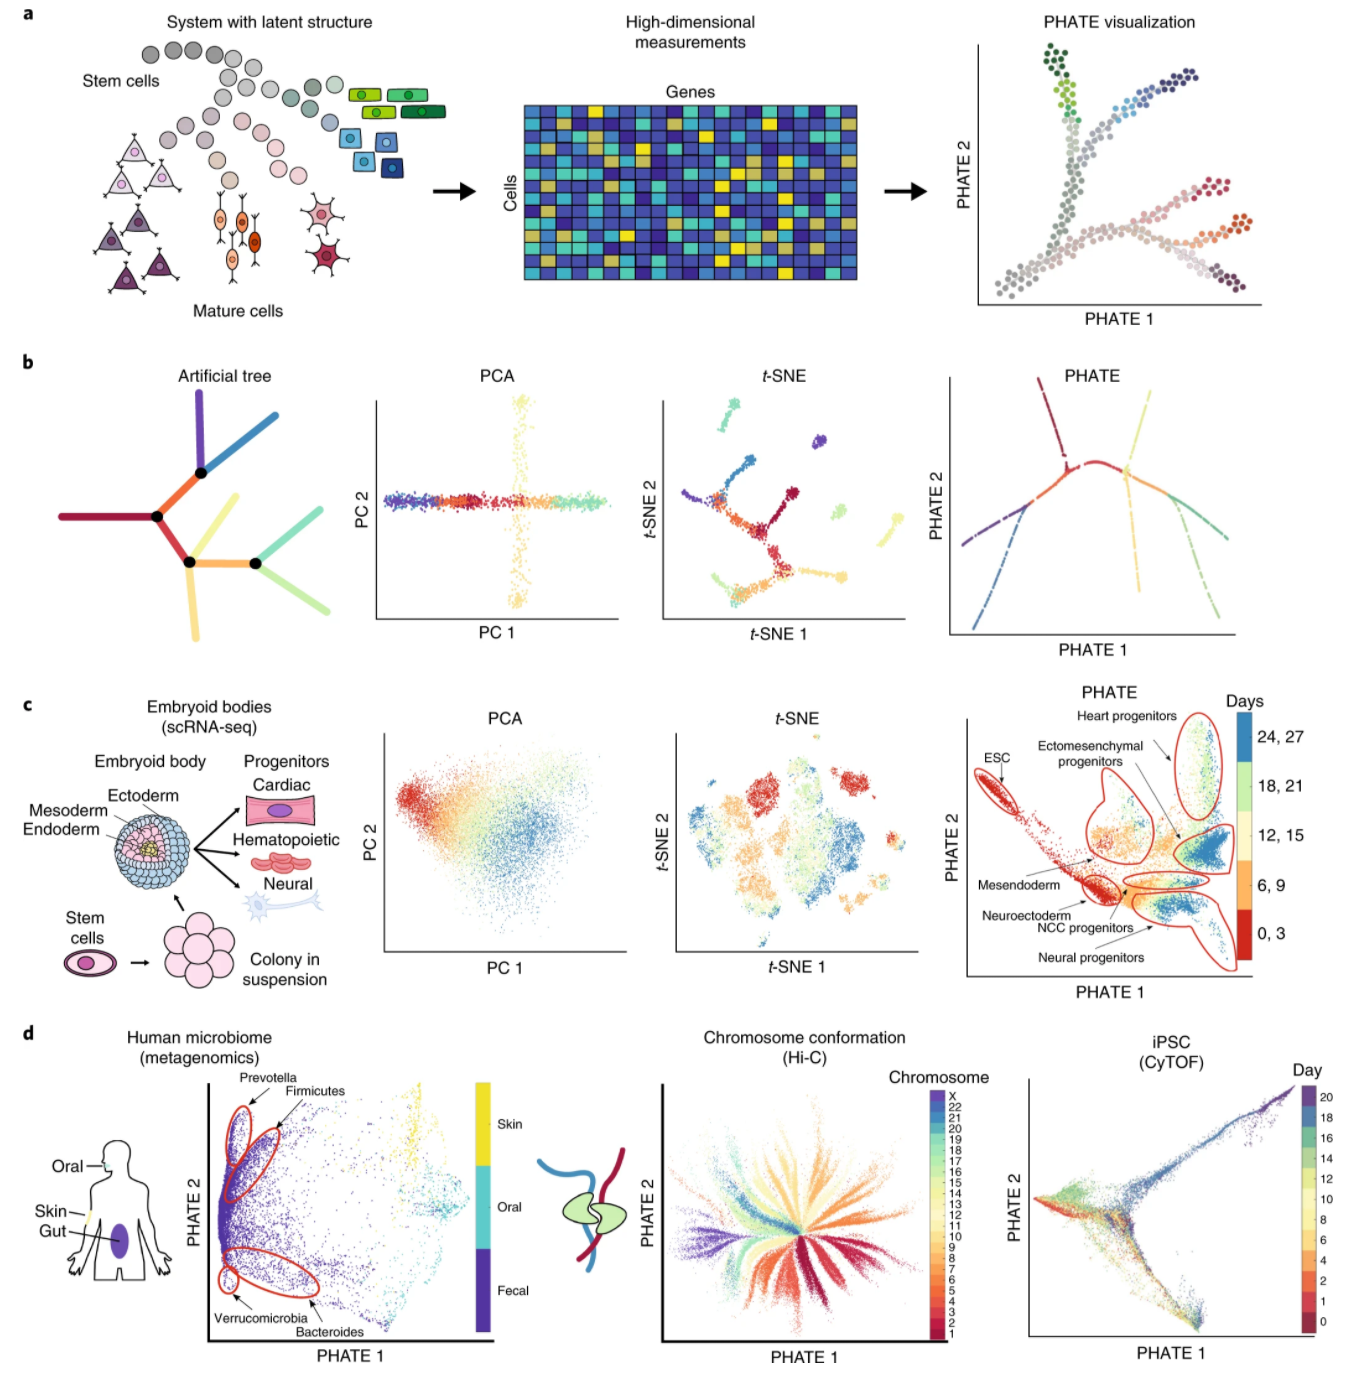
\includegraphics[width = 0.5\linewidth]{PKU_Slide/chaps/72b09f03212506c570b1ef2ecef54ad.png}
        \caption{Overview of PHATE and its ability to reveal structure in data.}
        % \label{fig:my_label}
    \end{figure}
\end{frame}

\begin{frame}{PHATE}
    \begin{figure}
        \centering
        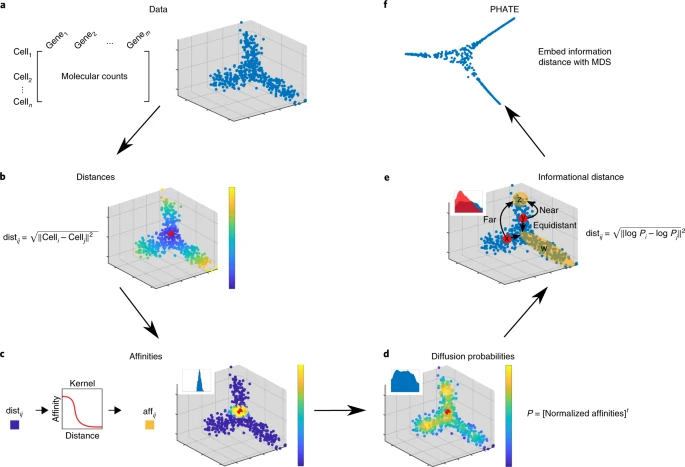
\includegraphics[width = 0.7\linewidth]{PKU_Slide/chaps/479317a57c2a602f4e3ad4fd4f9204d.png}
        \caption{Overview of PHATE and its ability to reveal structure in data.}
        % \label{fig:my_label}
    \end{figure}
\end{frame}

\begin{frame}{PHATE}
    \begin{figure}
        \centering
        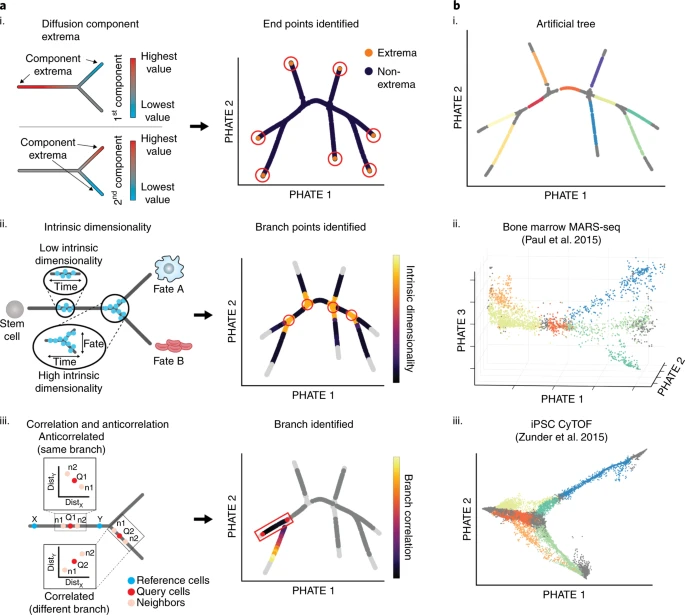
\includegraphics[width = 0.6\linewidth]{PKU_Slide/chaps/9fe8b62ea82aa486ec1552e89538aec.png}
        \caption{Extracting branches and branchpoints from PHATE.}
        % \label{fig:my_label}
    \end{figure}
\end{frame}

\begin{frame}{小结}
\begin{enumerate}
    \item 相较于PCA等方法,基于流形上扩散过程的\textit{扩散映射方法}能更好地提取出问题中的非线性特征,因为基于pairwise similarity可以更好地
    \item 该方法还可以优化社会调查指标的选取,只需要将$A$变成$A^T$... 
\end{enumerate}
\end{frame}

\begin{frame}{人类移动性与稳定性}
    Allee and everything.
    
    In the view of dynamical ecological system, epidemic spreading among $S$ urban patches can be understood as the interaction of infected subpopulations. Specifically, if we regard the infected population $I_{i}$ in an urban patch $i$ as a species, the spread of a disease results in the changes in the abundance. Thus the interaction of epidemic spreading can be described by a community matrix $M$, sized $S\times S$. The elements of $M$ changes dramatically with the spatial distribution of infection rate in a city, but can be regard as linear operator near a feasible equilibrium point, for an obvious example, $I_{i} = 0$ for $i$ in $1,2,\dots, S$.
    
\end{frame}